\documentclass[conference]{IEEEtran}
\IEEEoverridecommandlockouts
% The preceding line is only needed to identify funding in the first footnote. If that is unneeded, please comment it out.
\usepackage{cite}
\usepackage{amsmath,amssymb,amsfonts}
\usepackage{algorithmic}
\usepackage{graphicx}
\usepackage{textcomp}
\usepackage{xcolor}
\usepackage{hyperref}
\usepackage{cleveref}

\begin{document}

\title{An Interactive SMT Tactic in Coq using Abductive Reasoning}

\author{\IEEEauthorblockN{Arjun Viswanathan}
\IEEEauthorblockA{\textit{Dept. of CS} \\
\textit{University of Iowa}\\
Iowa City, USA \\
arjun.viswanathan23@gmail.com}
\and
\IEEEauthorblockN{Chantal Keller}
\IEEEauthorblockA{\textit{Laboratoire Méthodes Formelles} \\
\textit{Université Paris-Saclay}\\
Orsay, France \\
Chantal.Keller@lri.fr}
\and
\IEEEauthorblockN{Cesare Tinelli}
\IEEEauthorblockA{\textit{Dept. of CS} \\
\textit{University of Iowa}\\
Iowa City, USA \\
cesare-tinelli@uiowa.edu}
}

\maketitle

\begin{abstract}
  Interactive theorem provers (ITPs) and 
  automatic theorem provers (ATPs) offer 
  very different functionalities in 
  hardware and software verification. ITPs
  provide high assurances and low automation,
  while ATPs offer push-button proofs but are 
  less reliable. SMTCoq is a tool that allows 
  a user of the Coq ITP to delegate parts of 
  their proof to an SMT solver (an ATP), 
  without losing the proof guarantees of 
  the Coq kernel. It does this via a
  tactic, which tries to dispatch the current
  goal to an SMT solver. If the solver finds 
  a counterexample to the goal, it returns 
  this to the Coq user. We enhance this 
  integration with the SMT solver, allowing
  it instead to ask for facts that would 
  allow it to prove the goal, via abductive
  reasoning.
\end{abstract}

\begin{IEEEkeywords}
abduction, cvc5, SMTCoq, Coq, SMT
\end{IEEEkeywords}

\section{Introduction}
  Interactive theorem provers 
  (ITPs)~\cite{10.5555/1965123} are used to 
  prove logical properties in 
  various hardware and software verification tasks. 
  Interactive proofs are rigorous, but tedious, 
  involving elaborate sub-proofs of even simple 
  facts that could be automatically solved by automatic
  theorem provers (ATPs)
  such as SMT (satisfiability modulo 
  theories)~\cite{DBLP:reference/mc/BarrettT18} 
  solvers. Due to its proof approach, 
  adding an SMT (satisfiability modulo theories) 
  solver to the trust-base of an ITP is a liability 
  to its trustworthiness. 
  SMTCoq~\cite{10.1007/978-3-642-25379-9_12} is an 
  integration that achieves the best of both 
  worlds for certain logic fragments. Using one of 
  SMTCoq's tactics, a Coq~\cite{Thery2006} 
  user is able to dispatch goals 
  to a SAT/SMT solver without expanding Coq's trust-base. 
  SMTCoq achieves this by taking from the SMT 
  solver, along with its result, a certificate, and 
  using this certificate to construct a proof 
  term of the corresponding formula within Coq's 
  logic. 
  
  The traditional integration between Coq and 
  an SMT solver, say 
  cvc5~\cite{DBLP:conf/tacas/BarbosaBBKLMMMN22}, 
  via SMTCoq is as follows. The user 
  calls the \texttt{cvc5} tactic - provided by SMTCoq 
  in Coq - on a goal $G$, which asks cvc5 to prove
  $G$. If cvc5 succeeds, it also sends a proof 
  certificate, which SMTCoq uses to derive a proof 
  in Coq's logic using a process called computational
  reflection. If cvc5 fails because it found a 
  counterexample disproving $G$, it presents this 
  to the user, and the user is left to ponder whether 
  the counterexample was derived because the solver 
  didn't have enough information, or if $G$ is an 
  invalid statement.
  
  For cases where the solver finds a counterexample, 
  we introduce the \texttt{cvc5\_abduct} tactic which
  asks the SMT solver for a formula that would entail
  the goal $G$. With this tactic, we imagine a more 
  interactive session between the Coq user and the
  SMT solver, where the solver might be able to answer
  the question of what information it is lacking, in 
  order to prove the goal.
  

\section{Abduction via SyGuS}
  The cvc5 SMT solver performs abductive
  reasoning~\cite{DBLP:conf/cade/ReynoldsBLT20} 
  via syntax-guided synthesis
  (SyGuS)~\cite{6679385}. Given a 
  set of formulas $H$ (taken as a conjunction), 
  and a goal $G$, an abduct is a formula $\phi$ such
  that $H \land \phi \models G$. Furthermore, cvc5
  finds abducts modulo some theory $T$, so that 
  the entailment holds in $T$, and that 
  the abduct is consistent with the axioms in 
  $T$. Internally, since cvc5 uses SyGus to find
  abducts, the search-space for the abduct is 
  restricted syntactically by a grammar $R$, that may 
  be produced as a parameter to the abduction solver.
  
\section{The \texttt{cvc5\_abduct} Tactic}
  The \texttt{cvc5\_abduct} tactic takes a positive 
  integer parameter that indicates the number of 
  abducts the user wants from cvc5. The disjunction 
  of the abducts entails the goal, which is to 
  say that each abduct individually suffices to 
  entail the goal.
  
  \begin{figure}[htbp]
  	\centerline{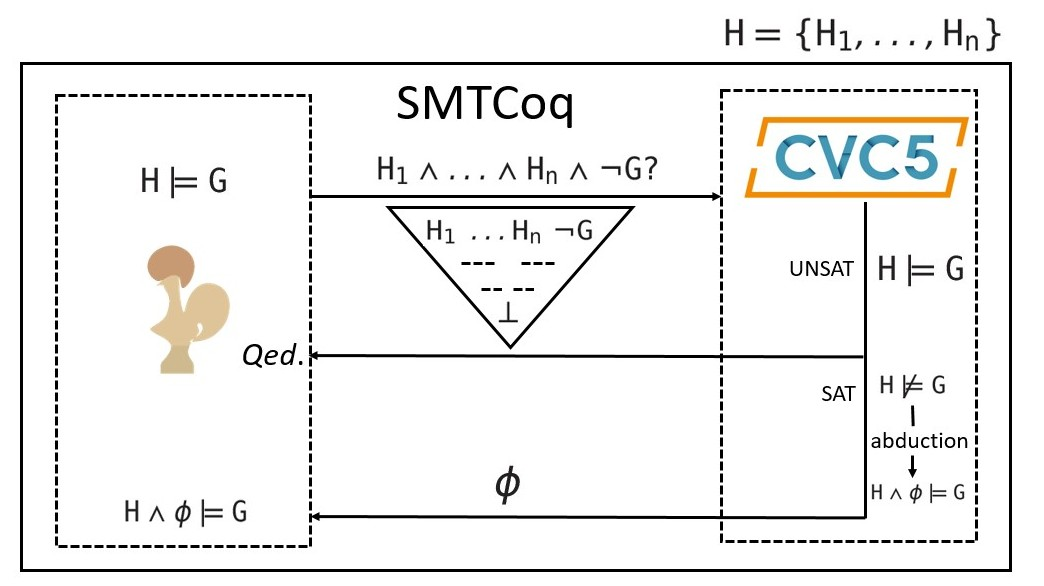
\includegraphics[scale=0.25]{abd.jpg}}
  	\caption{Interactions between Coq and cvc5 in 
  		SMTCoq.}
  	\label{fig}
  \end{figure}
  Fig.~\ref{fig} illustrates the enhancement 
  to the Coq-cvc5 integration that abduction 
  provides.
  Notice that a proof goal in Coq turns to an 
  unsatisfiability goal in cvc5. The proof 
  certificate returned by cvc5 is a tree that 
  derives the empty clause ($\bot$) from the 
  negation of the input, proving its 
  unsatisfiability. In cases where the SMT solver
  finds the negation of the goal to be satisfiable, 
  our tactic provides an alternative to 
  counterexamples, where cvc5 returns an abduct 
  $\phi$.
  
  In the following, we present an example of how
  this enhancement may be used. Suppose our Coq 
  development 
  contains a binary function \texttt{f} of type 
  \texttt{Z $\to$ Z $\to$ Z} (where \texttt{Z} is
  Coq's integer type), and many facts
  about \texttt{f}. We use the \texttt{cvc5} tactic 
  to ask the SMT solver to prove
  the following goal about \texttt{f}:
  \begin{center}
  	\texttt{forall (x y z : Z), x = y + 1}\\ 
  	\hspace{2cm}$\to$\texttt{(f y z) = f z (x - 1).}
  \end{center}
  The solver returns the following counter-example:
  \begin{center}
  	\texttt{f = $\lambda$ x, y $\to$ x}\\
  	\texttt{x = 1, y = 0, z = 1}
  \end{center}
  Instead of trying to determines the facts about 
  $f$ that would eliminate this and future 
  counter-examples, the user may invoke the 
  abduction solver via \texttt{cvc5\_abduct 3}
  tactic, which presents 3 abducts:
  \begin{center}
  	\texttt{z = y}\\
  	\texttt{z + 1 = x}\\
  	\texttt{f z y = f y z}
  \end{center}
  The third abduct might suggest to the user that 
  cvc5 only needs to know that the function is 
  commutative to prove the goal, and a subsequent 
  call to the \texttt{cvc5} tactic, with a proof
  of the commutativity of \texttt{f} (the SMTCoq 
  tactics allow for hypotheses to be passed 
  as arguments) would successfully close the proof.

\section{Conclusion and Future Work}
  We have extended SMTCoq by adding to its traditional
  set of proof tactics, 
  a more interactive tactic called \texttt{cvc5\_abduct}.
  When cvc5 finds a goal to be invalid, this tactic 
  presents an alternative to presenting counterexamples ---
  it relies on the abductive capabilities of cvc5 
  to present fact(s) that would entail the goal, to the 
  user. With tools that deal with integrating ATPs and
  ITPs such as hammers~\cite{10.1007/978-3-642-22438-6_11}
  \cite{article}, a good premise selection strategy
  is important to avoid either overloading the ATP with
  too many facts, or conversely supplying it with 
  insufficient facts to solve the 
  goal~\cite{DBLP:journals/jar/AlamaHKTU14}
  \cite{10.1007/978-3-642-31365-3_30}. With the 
  abduction tactic, 
  we imagine the ATP as being part of this premise 
  selection process.
  
  The development of the \texttt{cvc5\_abduct} tactic
  is still under development. There is a version that
  works in a branch, but only under certain restrictive
  parameters. Our first goal in this project is to 
  lift these restrictions and have a working version 
  of the tactic that is available in an SMTCoq release.
  Beyond that, there are many ways in which the 
  interaction with the abduction solver could be 
  improved. Currently, 
  we don't modify the default grammar that
  cvc5 selects to produce abducts, one that 
  contains rules for the generating the 
  entire language
  under consideration. A combination of allowing 
  grammar selection by the user and using automatic
  methods to reduce the language generated by the 
  grammar would allow for better abducts.
  
  The entire abduction pipeline is implemented 
  manually now, where the Coq user looks at the set 
  of abducts from the solver and 
  uses their understanding of the imported libraries
  and other available facts and selects any
  facts that may be implied by an abduct. One 
  can imagine automating this process using 
  a smarter tactic that is able to search 
  the open Coq libraries for facts that 
  match the abducts and automatically complete 
  the proof by including those facts.

\bibliographystyle{IEEEtran}
\bibliography{generic}

\end{document}
